%Para hacer informe con portada utilizamos report

\documentclass[12pt]{report}

\usepackage[a4paper]{geometry}
\usepackage[myheadings]{fullpage}
\usepackage{fancyhdr}
\usepackage{lastpage}
\usepackage{graphicx, wrapfig, subcaption, setspace, booktabs}
\usepackage[T1]{fontenc}
\usepackage[font=small, labelfont=bf]{caption}
\usepackage{fourier}
\usepackage[protrusion=true, expansion=true]{microtype}

%Paquete para hipervinculos
\usepackage[colorlinks=true]{hyperref}
\hypersetup{
    colorlinks=true,
    linkcolor=black,
    filecolor=black,      
    urlcolor=blue,
}

%Para qué los subtítulos aparezcan en español
\usepackage[spanish]{babel}
\usepackage[utf8]{inputenc}
\usepackage{sectsty}
\usepackage{url, lipsum}
\usepackage{tabularx}
\usepackage{float}

%--------------------------------------------------
%Para agregar citas en apa
%Para citar se usa el comando \cite{}
%Las referencias se modifican en el archivo sample.bib
\usepackage{apacite}
%----------------------------------------------

\newcommand{\HRule}[1]{\rule{\linewidth}{#1}}
\onehalfspacing
\setcounter{tocdepth}{5}
\setcounter{secnumdepth}{5}

%-------------------------------------------------------------------------------
%Encabezado y pie de pagina y numeracion
%\fancyhead para encabezado
%\fancyfoot para pie de pagina
% L para izquierda, left
% R para derecha, right
% C para centro, center
%-------------------------------------------------------------------------------
%\pagestyle{fancy}
%\fancyhf{}
%\setlength\headheight{15pt}
%\fancyhead[L]{\chaptername \ \thechapter} 
%\fancyhead[R]{UNMSM}
%\fancyfoot[R]{\thepage}
\usepackage{enumerate} 
\newcommand{\N}{\mathbb{N}}
\newcommand{\Z}{\mathbb{Z}}
\newcommand{\C}{\mathbb{C}}
\newcommand{\R}{\mathbb{R}}
\renewcommand{\qedsymbol}{$\square$}
\usepackage{graphicx}
\usepackage{setspace}
\usepackage{amsmath,amsthm,amssymb}
\usepackage[left= 3cm, right=3cm, top=2.5cm, bottom=2.5cm ]{geometry}


\doublespacing
\onehalfspace
\singlespace
\spacing{1.5}
\newtheorem{obs}{{Observación}}[section]
\newtheorem{defi}{Definición}[section]
\newtheorem{prop}{Proposición}[section]
\newtheorem{lemma}{Lema}[section]
\newtheorem{teo}{Teorema}[section]
\newtheorem{ejem}{Ejemplo}[section]
\newtheorem{cor}{Corolario}[section]


\begin{document}


%----------------------------------------------------------------------------------------
%	PORTADA
%----------------------------------------------------------------------------------------

\begin{titlepage}
 
\begin{center}
 
 {\large \bf UNIVERSIDAD NACIONAL MAYOR DE SAN MARCOS}\\
 
{\large FACULTAD DE CIENCIAS MATEMÁTICAS}\\{\large E.A.P. DE MATEMÁTICAS}\\[2.0cm]



\vspace{1cm}
\title{} % titulo de tu tesis para latex
{\bf \Large Propiedades Dinámicas de la Transformación de Gauss }\\[1.5cm] % titulo de tu tesis

{TESINA}\\[0.5cm]
{PARA OPTAR EL GRADO DE BACHILLER EN MATEMÁTICAS}\\[1.5cm]
 
\vspace{2cm} 

        
        {\large \textbf{ AUTORA }}\\
        
        \vspace{5mm}
        
        {\Large Fiorela Azahuanche Falcón}
        
        \vspace{50mm}
        
        
        
        {\Large \textbf{ Lima,Perú }}\\
        
        \vspace{3mm}
        {\Huge \textbf{2021}}
\end{center}

\end{titlepage}

\newpage
\newpage
%----------------------------------------------------------------------------------------
%	Resumen
%----------------------------------------------------------------------------------------
\renewcommand{\thepage}{\Roman{page}}
\begin{titlepage}

\begin{flushleft}
{\large \bf RESUMEN}
\end{flushleft}
\textit{En el presente trabajo, estudiamos sobre las fracciones continuas y su relación con la transformación de Gauss. Presentaremos como resultado las propiedades dinámicas de la Transformación de Gauss.}
\\
\\
$\begin{array}{cc} \textbf{Palabras claves:}
     & \text{Fracciones continuas.}  \\
     & \text{Transformación de Gauss.}\\
     & \text{Propiedades dinámicas.}
\end{array}$ % agregar tu dedicatoria
\end{titlepage}


%----------------------------------------------------------------------------------------
%	Abstract
%----------------------------------------------------------------------------------------

\begin{titlepage}

\begin{flushleft}

{\large \bf ABSTRACT}
\end{flushleft}
\textit{In this work, we study about continuous fractions and their relationship with the Gauss map. We will present the dynamic properties of the Gauss map as a result.}
\\
\\
$\begin{array}{cc} \textbf{Keywords:}
     & \text{Continuos fractions.}  \\
     & \text{Gauss map.}\\
     & \text{Dynamic properties.}
\end{array}$% agregar tu dedicatoria
\end{titlepage}

%----------------------------------------------------------------------------------------
%	TABLA DE CONTENIDOS
%--------------------------------------------------------------------------------------- 
\tableofcontents
\cleardoublepage
%\makegloss
\newpage

\renewcommand{\thepage}{\arabic{page}}
\setcounter{page}{1}

\chapter{Fracciones Continuas y Transformación de Gauss}
    \section{Expansión en Fracciones Continuas}
\begin{defi}
Una fracción continua es una fracción de la forma
$$
a_{0}+\cfrac{1}{a_{1} + \cfrac{1}{a_{2} + \ldots}}
$$
donde $a_{0}$ es un entero y los otros números $a_{n}$ con $n\geq1$ son números naturales.
\\

En lugar de escribir un número usando estas fracciones, es más común escribirlo de esta forma $a_{0}+[a_{1}, a_{2}, \ldots]$.

Los números $a_{0},a_{1},a_{2},\ldots$ se llaman los cocientes de la fracción continua y a los 
$$a_{0}+[a_{1}]=a_{0}+\frac{1}{a_{1}}$$
$$a_{0}+[a_{1},a_{2}]=a_{0}+\cfrac{1}{a_{1}+\cfrac{1}{a_{2}}}
$$
$$
\vdots
$$
se llaman reducidas.
\end{defi}

Plantearemos el siguiente teorema sin ninguna prueba, con el fin de enumerar algunas propiedades de las fracciones continuas:

\begin{teo}
Sea $x\in\mathbb{R}$ arbitrario:
\begin{itemize}
    \item[(a)] El número x tiene expansión en fracción continua.
    \item[(b)] Toda fracción continua converge.
    \item[(c)] La expansión en fracción continua de x es finita si y solo si x es racional.
    \item[(d)] La expansión en fracción continua de x es única si y solo si x es irracional.
\end{itemize}
\end{teo}
\begin{proof}
En \cite{Portugues}.
\end{proof}
\begin{ejem}
Veamos algunos números escritos en su expansión en fracción continua:
\begin{itemize}
    \item $\frac{22}{3}= 7 + \frac{1}{3} = 7+[3] \text{ pero también }\frac{22}{3}= 7 + \cfrac{1}{2 + \cfrac{1}{1}} = 7+[2,1]$
    \\
    
    De aquí notamos que la expansión de los racionales no es única.
    \item $\sqrt{2}=1+[2,2,2,2,\ldots]$, donde $a_{k}=2$ para todo $k\neq0$.
    \item $\pi=3+[3,7,15,1,292,1,1,1,2,1,3,1,14,\ldots]$, donde no hay un comportamiento regular aparente en sus cocientes.
\end{itemize}
\end{ejem}
\\
Surge la siguiente pregunta ¿cómo se halla la expansión en fracción continua de un número irracional? Esto será respondido más adelante y comprendido mediante el Ejemplo 1.2.1.

\begin{defi}
Sea $x\in\mathbb{R}$. Denotaremos como
\begin{itemize}
    \item El número entero $a_{n}(x)$ es el n-ésimo cociente de x.
    \item El número racional $a_{0} + [a_{1}(x), \ldots, a_{n}(x)]=\cfrac{p_{n}(x)}{q_{n}(x)}$ es la n-ésima reducida de $x$.
\end{itemize}
\end{defi}
\\
\\
Por otro lado, para probar la convergencia de las reducidas el primer paso es ver las propiedades de las reducidas de un número x, la cual verifican las siguientes propiedades aritméticas (Propiedades (A),(B),(C)).
\\

A continuación fijaremos $x$ y, para simplificar la notación, escribimos $a_{i}, p_{i} \text{ y } q_{i}$ en lugar de $a_{i}(x), p_{i}(x) \text{ y } q_{i}(x)$ cuando no es necesario especificar el número x.
\\

Por convención, escribiremos
$$
q_{-1}(x)=0\text{ , } p_{0}(x)=a_{0} \quad\text{ y }\quad p_{-1}(x)=q_{0}(x)=1
$$
\begin{prop}
\textbf{(Propiedades de las reducidas)}
\begin{itemize}
    \item[(A)] Para todo $n\geq1$ se verifica
    $$
    p_{n}=a_{n}p_{n-1}+p_{n-2} \quad \text{ y }\quad q_{n}=a_{n}q_{n-1}+q_{n-2}
    $$
    \item[(B)] Para todo $n\geq0$,
    $$(I)\quad p_{n-1}q_{n} - p_{n}q_{n-1}=(-1)^{n}$$
    $$
    (II)\quad x=\frac{p_{n} + (T^{n}(x))p_{n-1}}{q_{n}+(T^{n}(x))q_{n-1}}
    $$
    \item[(C)] Para todo $n\geq2$ se verifica 
    $$
    p_{n}(x)\geq2^{(n-2)/2} \quad\text{ y }\quad q_{n}(x)\geq2^{(n-1)/2}
    $$
\end{itemize}
\label{ProRed}
\end{prop}
\begin{proof}
En \cite{Portugues}.
\end{proof}

\begin{obs}
Notemos que la Propiedad (B) garantiza que cualquier divisor común de $p_{n}$ y $q_{n}$ debe ser también un divisor de $\pm$1. Por tanto, los números $p_{n}$ y $q_{n}$ son primos entre sí y la fracción $\cfrac{p_{n}}{q_{n}}$ es irreducible.
\end{obs}
\\
Por último recordemos la definición de parte entera.

\begin{defi}
Denotamos como $\left\lfloor x\right\rfloor$ a la parte entera de x, esto es, $\left\lfloor x\right\rfloor=n$ tal que $n \leq x< n+1$ con $n\in\mathbb{Z}.$
\end{defi}

    \section{Transformación de Gauss}
El sistema que se presentará a continuación (extraído de \cite{Viana}) está relacionado con otro importante algoritmo en Teoría de números, que es la expansión de un número en fracción continua cuyo origen se remonta al problema de hallar la mejor aproximación racional para un número real cualquiera. Vamos a describir ese algoritmo:\\

Dado un número $x \in(0,1),$ sean
\[
a_{1}=\left\lfloor\cfrac{1}{x}\right\rfloor \quad y \quad T_{1}=\cfrac{1}{x}-a_{1}
\]
Note que $a_{1}$ es un número natural y $T_{1} \in[0,1)$ entonces se tiene:
\[
x=\cfrac{1}{a_{1}+T_{1}}
\]
Suponiendo que $T_{1}$ $\neq 0$, podemos repetir el proceso , definiendo
\[
a_{2}=\left\lfloor\cfrac{1}{T_{1}}\right\rfloor \quad y \quad T_{2}=\cfrac{1}{T_{1}}-a_{2}
\]
Entonces 
\[
T_{1}=\cfrac{1}{a_{2}+T_{2}} \quad y \quad por \quad tanto \quad x=\cfrac{1}{a_{1}+\cfrac{1}{a_{2}+T_{2}}}
\]
Por recurrencia, para cada $n \geqslant 1$ tal que $T_{n-1} \in(0,1)$ se define
\[
a_{n}=\left\lfloor\cfrac{1}{T_{n-1}}\right\rfloor \quad y \quad T_{n}=\frac{1}{T_{n-1}}-a_{n}
\]
y se tiene: 
\begin{equation}
    x=\cfrac{1}{a_{1}+\cfrac{1}{a_{2}+\cfrac{1}{\ldots+\cfrac{1}{a_{n}+
    T_{n}}}}}
    \label{equa1}
\end{equation}

Se puede mostrar que la sucesión
\begin{equation}
    \alpha_{n} = \cfrac{1}{a_{1}+\cfrac{1}{a_{2}+\cfrac{1}{\ldots+\cfrac{1}{a_{n}}}}}
    \label{equa2}
\end{equation}
converge para $x$ cuando $n\to\infty$ y es usual traducir este hecho escribiendo
\begin{equation}
    x=\cfrac{1}{a_{1}+\cfrac{1}{a_{2}+\cfrac{1}{\ldots+\cfrac{1}{a_{n}+\cfrac{1}{\ldots}}}}}
    \label{equa3}
\end{equation}
que es llamada la expansión en fracción continua de $x$.

\begin{obs}
Notemos que la sucesión $\{\alpha_{n}\}_{n}$ definida en (\ref{equa2}) consiste de los números racionales. De hecho, estos son los números racionales que mejor aproximan al número $x$, en el sentido de que $\alpha_{n}$ está más próximo de $x$ que de cualquier otro número racional con denominador menor o igual que el denominador de $\alpha_{n}$ (escrito en su forma irreducible.)
Es decir,
$$
\alpha_{n}=[a_{1},a_{2},a_{3},\ldots,a_{n}]=\cfrac{p_{n}}{q_{n}}
$$
Sea $x=[a_{1},a_{2},a_{3},\ldots]$ una fracción continua infinita. Por la definión de aproximación diofántica $k\geq1$ y $1<q_{n}<k$ entonces:
$$
0<\left|x-\cfrac{p_{n}}{q_{n}}\right|<\frac{1}{kq_{n}}
$$
\end{obs}

\begin{obs}
Observemos también que para obtener (\ref{equa3}) suponemos que $T_{n}\in (0,1)$ para todo $n\in\mathbb{N}.$ Si encontramos algún $T_{n}=0$, el proceso para en ese momento y consideramos (\ref{equa1}) la expansión en franción continua de x. Claro que esto último caso ocurre solamente si x es un número racional.
\end{obs}

Ahora, el algoritmo de expansión en fracción continua esta conectado con el sistema dinámico en el intervalo [0,1) que vamos definir a continuación.

\begin{defi}
La Transformación de Gauss es definida por

\[
T:[0,1) \rightarrow[0,1)\quad,\quad T(x)=\left\{\begin{array}{c}
\cfrac{1}{x}-\left\lfloor\cfrac{1}{x}\right\rfloor, \text{ si x } \neq 0  \\\\
0, \text{ si x }  = 0
\end{array}\right.
\]
Definimos $T^{0}(x)=x$ e inductivamente $T^{i+1}(x)=T(T^{i}(x))$.
\end{defi}

\begin{obs}
Un número $x\in (0,1)$ es irracional si y solamente si $T(x)$ es irracional. Por tanto, un número $x$ es irracional si y solamente si, $T^{n}(x)$ es irracional (luego no nulo) para todo $n\geq0.$
\label{obs2}
\end{obs}

Además, el gráfico de $T$ puede ser esbozado fácilmente, a partir de la siguiente observación:
\begin{obs}
Para todo $x$ en cada intervalo $I_{k}=\left(\frac{1}{k+1},\frac{1}{k}\right]$, $k\geq1$, consideramos la parte entera de 1/x igual a k, por tanto, T(x)=1/x - k. Ver la Figura \ref{fig1}.
\end{obs}
\begin{figure}[h]
    \centering
    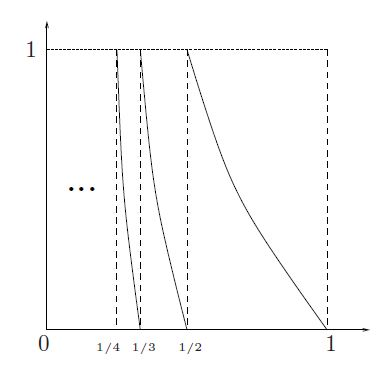
\includegraphics[width=10cm]{chapter1/TG.JPG}
    \caption{Gráfica de la Transformación de Gauss.}
    \label{fig1}
\end{figure}

\break

\begin{ejem}
\textbf{(Expansión de $\sqrt{3}$)} Probemos que $1+[1,2,1,2,\ldots]$ es la expansión en fracción continua de $\sqrt{3}$. Es decir, los cocientes de $\sqrt{3}$ forman una sucesión periódica, donde
$$
a_{2i+1}(\sqrt{3})=1 \quad y \quad a_{2i+2}(\sqrt{3})=2,
$$
para todo $i\geq0$.
Considerando $a_{0}(\sqrt{3})=\lfloor\sqrt{3}\rfloor=1.
$

\end{ejem}
\begin{proof}
Tenemos $a_{0}=\lfloor\sqrt{3}\rfloor=1$ y aplicamos la transformación de Gauss a $y = \sqrt{3}-1 \in (0,1)$,
$$
a_{1}(y)=\left\lfloor\frac{1}{y}\right\rfloor=\left\lfloor\frac{1}{\sqrt{3}-1}\right\rfloor=\left\lfloor\frac{\sqrt{3}+1}{(\sqrt{3}-1)(\sqrt{3}+1)}\right\rfloor=\left\lfloor\frac{\sqrt{3}+1}{2}\right\rfloor=1.
$$
Para calcular $a_{2}(y)$,
$$
a_{2}(y)=\left\lfloor\frac{1}{T(y)}\right\rfloor=\left\lfloor\frac{1}{\frac{1}{y}-\left\lfloor\frac{1}{y}\right\rfloor}\right\rfloor=\left\lfloor\frac{1}{\frac{\sqrt{3}+1}{2}-1}\right\rfloor=
$$
$$
=\left\lfloor\frac{2}{\sqrt{3}-1}\right\rfloor=\left\lfloor\frac{2(\sqrt{3}+1)}{2}\right\rfloor=\left\lfloor\sqrt{3}+1\right\rfloor=2.
$$
Para calcular $a_{3}(y)$,
$$
a_{3}(y)=\left\lfloor\frac{1}{T^{2}(y)}\right\rfloor=\left\lfloor\frac{1}{\frac{1}{T(y)}-\left\lfloor\frac{1}{T(y)}\right\rfloor}\right\rfloor=\left\lfloor\frac{1}{\sqrt{3}+1-2}\right\rfloor=
$$
$$
=\left\lfloor\frac{1}{\sqrt{3}-1}\right\rfloor=\left\lfloor\frac{\sqrt{3}+1}{2}\right\rfloor=1.
$$
Observemos que el proceso de calcular los cocientes $a_{i}(y)$ es el mismo que el de determinar las imágenes de $T^{i}(y)$. En el cálculo anterior obtuvimos
$$
\frac{1}{y}=\frac{1}{T^{0}(y)}=\frac{\sqrt{3}+1}{2}\quad,\quad \frac{1}{T^{1}(y)}=\sqrt{3}+1.
$$
Por inducción tendríamos que:
$$
\frac{1}{T^{2i}(y)}=\frac{\sqrt{3}+1}{2}\quad,\quad\frac{1}{T^{2i+1}(y)}=\sqrt{3}+1.
$$
Entonces para los $a_{i}$ tendríamos
$$
a_{2i+1}(y)=\left\lfloor\frac{1}{T^{2i}(y)}\right\rfloor = \left\lfloor\frac{\sqrt{3}+1}{2}\right\rfloor=1,
$$
$$
a_{2i+2}(y)=\left\lfloor\frac{1}{T^{2i+1}(y)}\right\rfloor = \left\lfloor\frac{\sqrt{3}+1}{2}\right\rfloor=2
$$
Entonces $y=\sqrt{3}-1=[a_{1},a_{2},a_{3},\ldots]$, entonces $\sqrt{3}=1+[a_{1},a_{2},a_{3},\ldots]$. Por tanto, la expansión en fracciones continuas de $\sqrt{3}$ es dada por $1+[1,2,1,2,\ldots]$.
\end{proof}

Continuando con el estudio de las expansiones en fracción continua de un número real (el caso interesante es el caso de los número irracionales). Hemos visto que a cada número irracional $x$ le asociamos usando la transformación de Gauss, su sucesión infinita $\{a_{k}\}_{k\geq0}$ de cocientes. 
\\

Donde un resultado importante será el siguiente Teorema que afirma que la sucesión de cocientes de un número irracional es infinita y que toda sucesión infinita de números naturales es la sucesión de los cocientes de un único número irracional. Obtenemos así una correspondencia biunívoca entre los números irracionales y las sucesiones infinitas de los números naturales.
\\

Formularemos de forma precisa estos resultados. Denotando por $\Sigma_{\infty}$ el conjunto de las sucesiones infinitas de los números naturales, $j=\{j_{k}\}_{k\in\mathbb{N}}$, $j_{k}\in\mathbb{N}$ y por $\mathbb{I}_{(0,1)}$ el conjunto de los números irracionales del intervalo (0,1). Considere la transformación
$$
\mathfrak{G}:\mathbb{I}_{(0,1)}\longrightarrow\Sigma_{\infty} \quad,\quad \mathfrak{G}(x)=\{a_{k}(x)\}_{k}
$$
que asocia a cada número irracional $x$ con su sucesión de cocientes.

\begin{teo}
La función $\mathfrak{G}$ es una biyección.
\label{teo3-1}
\end{teo}

\begin{proof}\hfill
\begin{itemize}
    \item[]Afirmación 1.$\mathfrak{G}$ es inyectiva. \\
    En efecto, sean $x,y\in\mathbb{I}_{(0,1)}$ y supongamos $\mathfrak{G}(x)=\mathfrak{G}(y)$ entonces  $a_{n}(x)=a_{n}(y)$ para todo $n\in\mathbb{N}$ entonces, tendriamos que $$
    x=\displaystyle\lim_{n\to\infty}[a_{1}(x),\ldots,a_{n}(x)]=\displaystyle\lim_{n\to\infty}[a_{1}(y),\ldots,a_{n}(y)]=y
    $$
    Entonces $x=y$.
    \item[]Afirmación 2. $\mathfrak{G}$ es sobreyectiva.
    \\
    En efecto, consideramos cualquier sucesión de números naturales $\{a_{n}\}_{n\in\mathbb{N}}$. Existe $x\in\mathbb{I}_{(0,1)}$ y como todo número real se puede expresar como fracción continua, tenemos que $x=[a_{1},\ldots,a_{n},\ldots]$\\
    Ahora, como la expresión en fracción continua de un número irracional es único $$[a_{1},\ldots,a_{n},\ldots]=x=[a_{1}(x),\ldots,a_{n}(x),\ldots].$$
    entonces $a_{n}=a_{n}(x)$ para todo $n\in\mathbb{N}$  y por tanto $\mathfrak{G}(x)=\{a_{n}\}_{n\in\mathbb{N}}$
\end{itemize} 
\end{proof}

Tenemos que el teorema anterior establece una relación biunívoca entre los números irracionales $\mathbb{I}_{(0,1)}$ del intervalo (0,1) y las sucesiones infinitas de los números naturales $\mathbb{N}^{\mathbb{N}}$: $x\mapsto[a_{1}(x),\ldots,a_{k}(x),\ldots]$. Lo cual significa que los números irracionales se caracterizan por tener expansión en fracciones continuas infinitas. En el siguiente capítulo obtendremos un interesante resultado: un número irracional tiene expansión periódica (puramente periódica o periódica a partir de un determinado término) si y solamente si es solución de una ecuación algebraica de segundo grado. Un ejemplo de este tipo de número es el número aúreo que es una raíz de la ecuación $x^{2}-x-1=0$.
\newpage

\chapter{Dinámica de la Transformación de Gauss}
    \section{Itinerarios de la Transformación de Gauss}
En este capítulo, daremos una prueba dinámica del Teorema \ref{teo3-1} donde estudiaremos los itinerarios de los puntos de $\mathbb{I}_{(0,1)}$ através de la transformación de Gauss, esto es determinaremos el intervalo $I_{k}$ que contiene el iterado i-ésimo de $x$ (en este caso $a_{i+1}(x)=k)$.
 \\
 
Recordemos que denotamos el conjunto de los números irracionales del intervalo (0,1) por $\mathbb{I}_{(0,1)}.$ Escribimos el intervalo (0,1) como la unión infinita de los intervalos 
$$
I_{k}=\left(\frac{1}{k+1},\frac{1}{k}\right], \quad k\geq1.
$$
Los extremos de los intervalos $I_{k}$ son precisamente los puntos de discontinuidad de la transformación de Gauss (excluida el origen). Recordemos que por la Observación \ref{obs2}, si $x\in\mathbb{I}_{(0,1)}$ entonces $T^{i}(x)\neq0$ para todo $i$ y por tanto $T^{i}(x)$ pertenece al interior de algún intervalo $I_{k}$ para todo $i\geq0$. Además se cumple lo siguiente:

\begin{prop}
Sea x $\in (0,1)$ un irracional y T es la transformación de Gauss. 
$$
a_{n}(x)=\left\lfloor\cfrac{1}{T^{n-1}(x)}\right\rfloor=k \Longleftrightarrow T^{n-1}(x)\in I_{k}
$$

\end{prop}

\begin{proof}\hfill
\\
($\Leftarrow$) Sea x $\in (0,1)$ un irracional con expansión en fracción continua $[a_{1}(x),a_{2}(x),\dots]$. Evaluando x en T, tenemos que \\

x=$\cfrac{1}{a_{1}(x)+\cfrac{1}{\ldots}}\Rightarrow T(x)=a_{1}(x)+\cfrac{1}{a_{2}(x)+\cfrac{1}{a_{3}(x)+\cfrac{1}{\ddots}}} - a_{1}(x)$
\\
\\

T(x)=$\left[a_{2}(x), a_{3}(x), \dots\right]=\cfrac{1}{a_{2}(x)+\cfrac{1}{a_{3}(x)+\cfrac{1}{\ddots}}}$
\\
\\

T$^{2}$(x)=$\left[a_{3}(x), a_{4}(x), \dots\right]=\cfrac{1}{a_{3}(x)+\cfrac{1}{a_{4}(x)+\cfrac{1}{\ddots}}}$
\\

$\quad\vdots$
\\

T$^{n-1}$(x)=$\left[a_{n}(x), a_{n+1}(x), \dots\right]=\cfrac{1}{a_{n}(x)+\cfrac{1}{a_{n+1}(x)+\cfrac{1}{a_{n+2}(x)+\cfrac{1}{\ddots}}}}$
\\

Se sigue inductivamente que, después de aplicar T exactamente $n-1$ veces el $a_{n}(x)$ es el cociente principal. 
\\

Podemos escribir $T^{n-1}(x)=\cfrac{1}{a_{n}(x)+m}$, \quad $m \in (0,1)$
\\

$\Rightarrow (T^{n-1}(x))^{-1}=a_{n}(x)+m< a_{n}(x) +1$, pues $m \in (0,1) $
\\

Además, como $a_{n}(x)\leq a_{n}(x)+m=(T^{n-1}(x))^{-1}$
\\

Entonces, $a_{n}(x)\leq (T^{n-1}(x))^{-1} < a_{n}(x)+1$
\\

i.e. $\cfrac{1}{a_{n}(x)+1}< T^{n-1}(x) \leq \cfrac{1}{a_{n}(x)}$
\\

De esto tenemos directamente que si $\cfrac{1}{k+1}< T^{n-1}(x) \leq \cfrac{1}{k}$, entonces $a_{n}(x)=k$ \\
\\
($\Rightarrow$) Consideramos $T^{n-1}(x) = [k,a_{n+1}(x),\dots]$, donde asumimos que $a_{n}(x) = k$
\\
Debido a la forma en que funciona $T$, sabemos que $0<[a_{n + 1}(x), a_{n + 2}(x), \dots] <1$ (i.e. no puede ser igual a ninguno de los extremos, porque eso implicaría que no existe $a_{n + 2}(x))$. Por lo tanto, podemos escribir $T^{n-1}(x)=\frac{1}{k+\alpha}$ con $\alpha \in (0,1)$. Tenemos lo mismo que para la vuelta, eso significa que $\frac{1}{k+1}< T^{n-1} \leq \frac{1}{k},$ es decir $T^{n-1}(x)\in I_{k}$.

De esta forma queda probada la proposición.
\end{proof}

\begin{obs}
La transformación de Gauss no es unifomemente expansiva, esto es, no existe $\lambda>1$ tal que $|T^{\prime}(x)|\geq\lambda>1$ para todo $x \in(0,1) - \left\{\frac{1}{k} : k\in\mathbb{N}\right\}$ (eliminamos exactamente los puntos de discontinuidad). En efecto, si $x\in I_{k}$, $T(x)=1/x - k$, k es la parte entera de $1/x$, así la derivada sería, $T'(x)= -1/x^2 < 0$. Luego, T es decreciente, es decir, si $x,y \in I_{k}$ y $x<y$ entonces, $T(x)>T(y)$.
\end{obs} 

\begin{obs}
Por la definición de T, tenemos que $T(I_{k})=[0,1)$ para todo $k\geq1$.
\end{obs}
\begin{defi}
Dados k,j $\in\mathbb{N}$, definimos $I_{k,j}$ como el subconjunto de $I_{k}$ tal que
$
T(I_{k,j})=I_{j} .
$
\label{defi3-2}
\end{defi} 
\begin{obs}
Como $T$ es estrictamente monótona decreciente en $I_{k}$, entonces es inyectiva y por tanto tiene inversa, es decir, $I_{k,j}=T^{-1}(I_{j})$. Además, desde que $T(I_{k})=[0,1)$, obtenemos que los conjuntos $I_{k,j}$ están bien definidos y que son intervalos no vacíos (intervalos cerrados a izquierda y abiertos a derecha).
\end{obs}
Veámoslo de esta manera:


$
\text{Sea } x=[a_{1},a_{2},\ldots] \text{, para } x \in I_{a_{1}} \Rightarrow T(x)=\frac{1}{x}-\underbrace{\left\lfloor\frac{1}{x}\right\rfloor}_{=a_{1}}=\frac{1}{x}-a_{1}
$ \\

$
T(x)=[a_{2},a_{3},\ldots] \text{, para } T(x) \in I_{a_{2}}\Rightarrow T^{2}(x)=\frac{1}{T(x)}-\underbrace{\left\lfloor\frac{1}{T(x)}\right\rfloor}_{=a_{2}}=\frac{1}{T(x)}-a_{2} \\
$

Como $T(x) \in I_{a_{2}}$ entonces $x\in T^{-1}(I_{a_{2}})=I_{a_{1},a_{2}}\subset I_{a_{1}}$.
\\

Tenemos que, para $x\in I_{a_{1},a_{2}}$ consideramos la parte entera de $1/T(x)$ igual a $a_{2}$  por tanto $T^{2}(x)=\frac{1}{T(x)}-a_{2}$.
Véase la figura \ref{TG2}.

\begin{figure}[h]
    \centering
    \includegraphics[width=9cm]{chapter2/intervalos de segunda generación.jpg}
    \caption{Intervalos de segunda generación}
    \label{TG2}
\end{figure}

\begin{prop}
La Transformación de Gauss tiene alguna expansividad uniforme: existe $\lambda>1$ tal que $(T^2)'(x)>\lambda$ para todo $x\in I_{a_{1}}$.
\end{prop}
\begin{proof}
En efecto, tenemos que $T(x)=\frac{1}{x} - a_{1}=\frac{1-a_{1}x}{x},\quad x\in I_{a_{1}}$.
\\
\\
$\Rightarrow T^{2}(x)=\frac{x}{1-a_{1}x}-a_{2},\quad x\in I_{a_{1},a_{2}}$ y $a_{2}$ es la parte entera de $\frac{x}{1-a_{1}x}$.
\\
\\
Así la derivada es, ($T^{2})^{\prime}(x)=\frac{1-a_{1}x-x(-a_{1})}{(1-a_{1}x)^2}=\frac{1}{(1-a_{1}x)^{2}},\quad x\in I_{a_{1},a_{2}}\subset I_{a_{1}}$.
\\
\\
$\Rightarrow x\in I_{a_{1}} \Rightarrow\frac{1}{a_{1}+1} <  x \leq \frac{1}{a_{1}} \Rightarrow -1 \leq -a_{1}x < \frac{-a_{1}}{a_{1}+1}$\\
\\
$\Rightarrow 0 \leq 1-a_{1}x < \frac{1}{a_{1}+1}$
\\
\\
$\Rightarrow 0 \leq (1-a_{1}x)^{2} < (\frac{1}{a_{1}+1})^{2}$
\\
\\
$\Rightarrow ({a_{1}+1})^{2}< \frac{1}{(1-a_{1}x)^{2}}=(T^{2})^{\prime}(x)$
\\
\\
Como $a_{1}\in\mathbb{N}$, entonces $({a_{1}+1})^{2}>1$, tomamos $\lambda=({a_{1}+1})^{2}$.
\\
\\
Luego, existe $\lambda>1$ tal que $(T^2)'(x)>\lambda$.
\\
Más aún, $T^{2}$ es creciente, pues, su derivada es mayor a cero. 
\end{proof}

\begin{prop}
Sea $k\in\mathbb{N}$ y para toda familia de $k$ números naturales $i_{1},i_{2},\ldots,i_{k}$, están definidos los intervalos no vacíos $I_{i_{1},\ldots,i_{k}}$ que verifican las siguientes propiedades:
\begin{enumerate}
    \item $I_{i_{1},\ldots,i_{k-1},i_{k}}\subset I_{i_{1},\ldots,i_{k-1}}$
    \item $T(I_{i_{1},\ldots,i_{k}})=I_{i_{2},\ldots,i_{k}}$ y
    \item $T^{k-1}(I_{i_{1},\ldots,i_{k-1},i_{k}})=I_{i_{k}}$ (luego, $T^{k}(I_{i_{1},\ldots,i_{k}})=[0,1)$)
\end{enumerate}
\label{PropInterval}
\end{prop} 

\begin{proof}
Probaremos por inducción sobre k. 
\begin{enumerate}
    \item[i)] Para k=2. Por la Definición \ref{defi3-2}, dado $I_{i_{2}}$ definimos $I_{i_{1},i_{2}}$ subconjunto de $I_{i_{1}}$ tal que $T(I_{i_{1},i_{2}})=I_{i_{2}}$ que vendría a ser la condición 1 y 2.
    \\
    Como $T(I_{i_{1},i_{2}})=I_{i_{2}}$ entonces $T^{2}(I_{i_{1},i_{2}})=T(I_{i_{2}})=[0,1)$ por lo que también tendríamos la condición 3.
    \item[ii)] (Hip. Inductiva) Para k=n es válido:
    \begin{itemize}
    \item[H1] $I_{i_{1},\ldots,i_{n-1},i_{n}}\subset I_{i_{1},\ldots,i_{n-1}}$
    \item[H2]
    $T(I_{i_{1},\ldots,i_{n}})=I_{i_{2},\ldots,i_{n}}$ y
    \item[H3] $T^{n-1}(I_{i_{1},\ldots,i_{n-1},i_{n}})=I_{i_{n}}$ (luego, $T^{n}(I_{i_{1},\ldots,i_{n}})=[0,1))$
    \end{itemize}
    \item[iii)]Veamos es válido para k=n+1. 
    \\
    En efecto, contruiremos los intervalos $I_{i_{1},\ldots,i_{n},i_{n+1}}$ de la etapa $n+1$. 
    \begin{itemize}
        \item Dados los números naturales $i_{1},\ldots,i_{n},i_{n+1}$ consideramos el intervalo $I_{i_{1},\ldots,i_{n}}$ y observamos que por $H3$,
        $$
        T^{n}(I_{i_{1},\ldots,i_{n}})=T(I_{i_{n}})=[0,1).
        $$
        
        Como la transformación $T^{n}$ es estrictamente mónotona (creciente si n es par y decreciente si n es impar) tenemos que los conjuntos $I_{i_{1},\ldots,i_{n+1}}$ están bien definidos y que son intervalos no vacíos.
        
        Ahora, por el primer paso de inducción, dado $I_{i_{n+1}} \text{ , existe } \\
        J\subset I_{i_{1},\ldots,i_{n}}$ tal que $T^{n}(J)=I_{i_{n+1}}$.
        
        Es suficiente tomar $I_{i_{1},\ldots,i_{n},i_{n+1}}=J$, entonces por construcción, $T^{n}(I_{i_{1},\ldots,i_{n},i_{n+1}})=I_{i_{n+1}}.$
        Además, $T^{n+1}(I_{i_{1},\ldots,i_{n},i_{n+1}})=T(I_{i_{n+1}})=[0,1)$.
        
        Lo que verifica la condición 3.
        \item Ahora de lo anterior teníamos que existe $J \subset I_{i_{1},\ldots,i_{n}}$ y como $J=I_{i_{1},\ldots,i_{n},i_{n+1}}$ entonces $I_{i_{1},\ldots,i_{n},i_{n+1}}\subset I_{i_{1},\ldots,i_{n}}$.
        Lo que verifica la condición 1.
        \item Queda probar la condición 2.
        
        Para cada $j$ $(1\leq j\leq n)$ denotamos por $T^{j}_{i_{1},\ldots,i_{n}}$ la restricción de $T^{j}$ al intervalo $I_{i_{1},\ldots,i_{n}}$. Estas transformaciones son inyectivas.
        
        Por la Definición \ref{defi3-2}, teníamos que $$T_{i_{1}}(I_{i_{1},i_{2}})=I_{i_{2}}\Rightarrow T^{-1}_{i_{1}}(I_{i_{2}})=I_{i_{1},i_{2}}\subset I_{i_{1}}$$
        $$
        \Rightarrow T^{-n}_{i_{1},\ldots,i_{n}}(I_{i_{n+1}})=I_{i_{1},\ldots,i_{n+1}}\subset I_{i_{1},\ldots,i_{n}}
        $$
        $$
        \Rightarrow T(I_{i_{1},\ldots,i_{n+1}})=T(T^{-n}_{i_{1},\ldots,i_{n}}(I_{i_{n+1}})) \subset T(I_{i_{1},\ldots,i_{n}})=I_{i_{2},\ldots,i_{n}}
        $$
        Por lo tanto, $T(I_{i_{1},\ldots,i_{n+1}})\subset I_{i_{2},\ldots,i_{n}}$.
        
        Luego,
        $$
        T_{i_{1}, i_{2} \ldots, i_{n}}^{-(n-1)}\left(I_{i_{n+1}}\right)=T_{i_{2}, \ldots, i_{n}}^{-(n-1)}\left(I_{i_{n+1}}\right)
        $$
        Así mismo tenemos,
        $$
        \begin{aligned}
        T\left(I_{i_{1}, \ldots, i_{n}, i_{n+1}}\right) &=T\left(T_{i_{1}, \ldots, i_{n}}^{-n}\left(I_{i_{n+1}}\right)\right)=T_{i_{1}, \ldots, i_{n}}^{-(n-1)}\left(I_{i_{n+1}}\right)=\\
        &=T_{i_{2}, \ldots, i_{n}}^{-(n-1)}\left(I_{i_{n+1}}\right)
        \end{aligned}
        $$
        
        Por otro lado, por H3,
        $$
        T^{n-1}\left(I_{i_{2}, \ldots, i_{n}, i_{n+1}}\right)=I_{i_{n+1}}
        $$
        Esto es,
        $$
        I_{i_{2}, \ldots, i_{n}, i_{n+1}}=T_{i_{2} \ldots, i_{n}}^{-(n-1)}\left(I_{i_{n+1}}\right)
        $$
        
        Por lo tanto,
        $$
        T\left(I_{i_{1}, \ldots, i_{n}, i_{n+1}}\right)=T_{i_{2} \ldots, i_{n}}^{-(n-1)}\left(I_{i_{n+1}}\right)=I_{i_{2}, \ldots, i_{n}, i_{n+1}}
        $$
    \end{itemize}
    Esto termina la construcción de los intervalos $I_{i_{1}, \ldots, i_{n}, i_{n+1}}$.
\end{enumerate}
De esa manera queda probada la proposición.
\end{proof}

A continuación relacionaremos los intervalos $I_{i_{1},\ldots,i_{n}}$ con los cocientes de la expansión en fracción continua.

\begin{prop}
Dado $x \in(0,1)$ sea $a_{i}(x)$ el i-esimo cociente de x. Entonces
$$
I_{i_{1}, \ldots, i_{n}}=\left\{x \in(0,1): i_{1}=a_{1}(x), \ldots, i_{n}=a_{n}(x)\right\}
$$
\label{teo3-2}
\end{prop}
\begin{proof}\hfill
\begin{itemize}
    \item[($\subseteq$)]Se probará por inducción sobre $n$.
    Consideramos
    $$
    x \in I_{i_{1}}=\left(\frac{1}{i_{1}+1}, \frac{1}{i_{1}}\right]\Rightarrow \cfrac{1}{i_{1}+1}<x\leq\frac{1}{i_{1}}\Rightarrow i_{1} \leq \frac{1}{x} < i_{1}+1
    $$
    $\Rightarrow \left\lfloor\frac{1}{x}\right\rfloor = i_{1}$ por la definición de parte entera.
    
    
    Además, recordemos que $a_{1}(x)=\left\lfloor\frac{1}{x}\right\rfloor=i_{1}$.
    
    
    Así tenemos la prueba para $n=1$. 
    \\
    \\
    Supangamos ahora la inclusión es verdadera para todo $1 \leqslant k \leqslant n$.
    \\
    i.e. $\quad x \in I_{i_{1},\ldots, i_{n}}  \Rightarrow i_{1}=a_{1}(x), \ldots, i_{n}=a_{n}(x)$ %por las propiedades de $I_{i_{1} \ldots, i_{k}}$
    \\
    \\
    Veamos se cumple para n+1 : 
    \\
    \\
    Consideramos
    $
    x \in I_{i_{1}, \ldots, i_{n+1}} \Rightarrow T(x) \in T\left(I_{i_{1}, \ldots, i_{n+1}}\right)
    $
    \\
    Por las Proposición \ref{PropInterval} condición (2), tenemos
    $$
    T(x) \in T\left(I_{i}, \ldots, i_{n+1}\right)=I_{i_{2}, \cdots, i_{n+1}}$$
    Por la hipótesis inductiva tendríamos:
    $$
    a_{1}(T(x))=i_{2}, \ldots, a_{n}(T(x))=i_{n+1}
    $$
    Además, $T^{n}\left(I_{{i_{1}}, \ldots, i_{n+1}}\right)=I_{i_{n+1}}$.
    \\
    \\
    Como $T^{n}(x) \in T^{n}\left(I_{i_{1}, \ldots, i_{n+1}}\right)=I_{i_{n+1}}$
    \\
    \\
    $\Rightarrow T^{n}(x)\in I_{i_{n+1}}$
    $\Rightarrow \quad \left\lfloor\cfrac{1}{T^{n}(x)}\right\rfloor=i_{n+1}$, donde $a_{n+1}(x)=\left\lfloor\cfrac{1}{T^{n}(x)}\right\rfloor$.
    \\
    \\
    Veamos $a_{n}(T(x))=a_{n+1}(x)$. En efecto, si $x=\left[a_{1,} \ldots, a_{n+1}, \ldots\right] \Rightarrow T(x)=\left[a_{2}, \ldots, a_{n+1}, \ldots\right]$
    \\
    entonces 
    \begin{equation}
    \begin{array}{l}
    a_{1}(T(x))=a_{2}(x)=i_{2}\\
    a_{2}(T(x))=a_{3}(x)=i_{3} \\
    \vdots \\
    a_{n-1}(T(x))=a_{n}(x)=i_{n} \\
    a_{n}(T(x))=a_{n+1}(x)=i_{n+1}
    \end{array}
    \label{equa4}
    \end{equation}
    Esto conluye la prueba de la inclusión ``$\subset$''.
    \item[($\supseteq$)] Para la otra inclusión se sigue de la definición de los intervalos $I_{i_{1}, \ldots, i_{n}}$ por inducción.
    \\
    \\
    $n=1: \quad a_{1}(x)=i_{1} \Longleftrightarrow \left\lfloor\cfrac{1}{x}\right\rfloor=i_{1} \Longleftrightarrow x \in I_{i_{1}}=\left(\frac{1}{i_{1}+1}, \frac{1}{i_{1}}\right]$
    \\
    \\
    (Hip.Ind.) Supongamos que es válido para las de longitud $n$.
    \\
    i.e. $a_{1}(x)=i_{1}, \ldots, a_{n}(x)=i_{n} \Rightarrow x \in I_{i_{1}, \ldots, i_{n}}$
    \\
    \\
    Veamos es válido para las de longitud $n+1$.
    \\
    \\
    Tomamos $x$ tal que $a_{1}(x)=i_{1}, \ldots, a_{n+1}(x)=i_{n+1} .$
    \\
    \\
    Por probar que $x \in I_{i_{1}, \ldots, i_{n+1}}$
    \\
    Por (\ref{equa4}) tenemos $a_{1}(T(x))=i_{2}, \ldots, a_{n}(T(x))=i_{n+1}$
    \\
    y por (Hip. Ind.) $T(x) \in I_{i_{2}, \ldots, i_{n+1}}=T\left(I_{j, \ldots, i_{n+1}}\right)$
    $\Rightarrow x \in I_{j, \ldots i_{n+1}}$ para algún $j$
    \\
    \\
    Vamos a probar que $j=i_{1}$. \\
    Supongamos lo contrario, que $j \neq i_{1} \Rightarrow I_{j} \cap I_{i_{1}}=\emptyset$
    \\
    \\
    Como $ I_{j, \ldots, i_{n+1}}\subset I_{j} \quad \wedge \quad x \in I_{i_{1}}$
    \\
    $\Rightarrow x \in I_{j}\quad \wedge \quad x \in I_{i_{1}}$
    \\
    $\Rightarrow x\in I_{j}\cap I_{i_{1}}$
    \\
    $\Rightarrow I_{j}\cap I_{i_{1}}\neq\emptyset$, la cual es una contradicción.
    \\
    Por lo tanto, $j=i_{1}$.

\end{itemize}
Por las dos inclusiones, tendríamos probada la proposición. 
\end{proof}

\begin{prop}
Dado una sucesión infinita $\{i_{k}\}_{k\in\mathbb{N}}$ de números naturales existe un único número (necesariamente irracional) $x \in(0,1)$ cuyos cocientes $\{ a_{k}(x)\}_{k\in\mathbb{N}}$ verifica $a_{k}(x)=i_{k}, \forall k$.
\label{teo3-3}
\end{prop}
\begin{proof}
Tenemos $x \in(0,1)$ cuyos cocientes son $\left\{a_{k}(x)\right\}_{k\in\mathbb{N}}$
\begin{equation*}
    \begin{array}{l}
    a_{1}(x)=i_{1} \Longleftrightarrow x \in I_{i_{1}}\\
    a_{1}(x)=i_{1}, a_{2}(x)=i_{2} \Longleftrightarrow x \in I_{i_{1}, i_{2}}\\
    a_{1}(x)=i_{1}, a_{2}(x)=i_{2}, a_{3}(x)=i_{3} \Longleftrightarrow x \in I_{i_{1}, i_{2}, i_{3}}
    \\
    \vdots
    \\
    a_{1}(x)=i_{1}, a_{2}(x)=i_{2}, \ldots, a_{n}(x)=i_{n} \Longleftrightarrow x \in I_{i_{1}, i_{2}, \ldots, i_{n}}
    \\
    \vdots
    \end{array}
    \end{equation*}
    Se observa que $x \in \displaystyle\bigcap_{k=1}^{\infty} I_{i_{1}, \ldots, i_{k}} \neq \emptyset$
    \\
    entonces por la Proposición \ref{teo3-2} se verifica $a_{k}(x)=i_{k}, \forall k \in \mathbb{N}$.
    \\
    La irracionalidad de x se sigue del hecho de que su representación en fracción continua es infinita y por tanto $T^{i}(x) \neq 0$,  $\forall i \geqslant 0$ de la Observación \ref{obs2}.
    \\
    La unicidad es equivalente a que la intersección $\displaystyle\bigcap_{k=1}^{\infty}I_{i_{1},\ldots,i_{k}}$ sea exactamente un punto.
    \\
    En efecto, supongamos por el absurdo que existen 2 puntos $x,y$ con $x<y$ en la intersección.
    \\
    Tenemos que $x, y$ son irracionales. Como el intervalo $[x, y]$ contiene números racionales, entonces por la Observación \ref{obs2}, existe $\ell\geq1$ tal que $0\in T^{\ell}([x,y])$.
    \\
    Por otro lado, por la Proposición \ref{PropInterval} condición (3), $\mathrm{T}^{\ell}([x, y])=[0,1)$.
    \\
    Como $T^{\ell}$ es estrictamente monótona.
    \\
    $\Rightarrow T^{\ell}(x)=0 \quad \vee \quad T^{\ell}(y)=0$
    \\
    $\Rightarrow x\in\mathbb{Q}$ $\vee$ $y\in\mathbb{Q}$, la cual es una contradicción.
    \\
    Luego, tiene exactamente un punto en la intersecuión.
    \\
    Por lo tanto, existe un único irracional $x\in(0,1)$ cuyos cocientes son $\{a_{k}\}_{k\in\mathbb{N}}$ que verifican $a_{k}(x)=i_{k}$, $\forall k$.
\end{proof}

    \section{Propiedades Topológicas}
En esta sección estudiaremos algunas propiedades topólogicas de la Transformación de Gauss: transitividad, topológicamente mixing, existencia de órbitas densas y la densidad de los puntos periódicos. Estas propiedades son resultado de la construcción de los intervalos $I_{[n]}=I_{i_{1},\ldots,i_{n}}$ de la sección anterior.

\begin{defi}
Considere un espacio métrico (X,d). Una función \\$f: X\rightarrow X$ es
\begin{itemize}
    \item Topológicamente transitiva: Si para todo par de conjuntos abiertos no vacíos U y V de X existe $n \in \mathbb{N}$ tal que $f^{n}(U)\cap V\neq\emptyset$.
    \item Topológicamente mixing: Si para todo par de conjuntos abiertos no vacíos U y V de X existe $k_{0}\in \mathbb{N}$ tal que se verifica $f^{n}(U)\cap V\neq\emptyset$ para todo $n\geq k_{0}$.
\end{itemize}

\end{defi}

\begin{obs}
Toda transformación topológicamente mixing es topológicamente transitiva. Sin embargo, existen transformaciones topológicamente transitivas que no son mixing. Los ejemplos más simples son las rotaciones irracionales del círculo, que obviaremos su estudio pero puede ser encontrado en \cite{Portugues}.
\end{obs}



\begin{prop}
La transformación de Gauss es topológicamente mixing.
\end{prop}

\begin{proof}
Consideremos dos abiertos no vacíos U y V de [0,1).
\\
Como todo intervalo abierto contiene infinitos intervalos $I_{i_{1}, \ldots, i_{k}}$.
\\
Existe un intervalo $I_{i_{1}, \ldots, i_{j}, k}$ contenido en U para $j$ suficientemente grande.
\\
Por la Proposición \ref{PropInterval} condición (3), obtenemos
\\
$$
\begin{array}{l}
T^{j}(I_{i_{1}, \ldots, i_{j},k})=I_{k}\\
T^{j+1}(I_{i_{1}, \ldots, i_{j},k})=T(I_{k})=[0,1)\\
T^{j+2}(I_{i_{1}, \ldots, i_{j},k})=T^{2}(I_{k})=T([0,1))=[0,1)\\
\vdots\\
\end{array}
$$
Por inducción, $\forall m\geq1$, $T^{j+m}(I_{i_{1}, \ldots, i_{j},k})=T^{m}(I_{k})=[0,1)\\$
$$
[0,1)=T^{j+m}\left(I_{i_{1}, \ldots, i_{j},k}\right)\subset T^{j+m}(U)$$
Luego, $T^{j+m}(U)=[0,1), \forall m \geqslant 1$
\\
Tomando $j=k_{0}$, tenemos $n=k_{0}+m\geq k_{0}$.
\\
Entonces, $T^{n}(U) \cap V=V \neq \emptyset ,\quad \forall n\geq k_{0}$.
\\
Por lo tanto, T es topológicamente mixing.
\end{proof} 

Tenemos que la transformación de Gauss es topológicamente mixing, lo que significa que iterando positivamente cualquier intervalo abierto $U$ (esto es, considerando las imágenes $T^{i}(U)$, $i\geq0$) los conjuntos $T^{i}(U)$ se distribuyen a lo largo de todo el intervalo de (0,1). Ahora, lo siguiente sería entender mejor esta distribución, la cual para ello se introduce herramientas ergódicas (probabilísticas) que se verían en un siguiente trabajo analizando las propiedades ergódicas de la transformación de Gauss. Además, de la proposición anterior, $T$ es transitiva, lo cual significa intuitivamente que la dinámica no se puede dividir en dos o más conjuntos porque todos sus elementos (iterados) van a estar mezclados de alguna manera, es decir, es indescomponible.
\\

\textbf{Escólio.} Dado cualquier conjunto abierto $U$ de $[0,1)$ existe $k>0$ tal que $T^{k}(U)=[0,1)$.
\\

Por otro lado, ciertas fracciones continuas, como
$$
\sqrt{11} = 3+[3,6,3,6,\ldots] = 3+[\overline{3,6}],
$$
son períodicos solo después de una determinado término. Y otras como
$$
\sqrt{11} +3 = [6,3,6,\ldots] = [\overline{6,3}],
$$
son periódicas desde el principio y se denominan fracciones continuas puramente periódicas.

Por ello, introducimos una notación para la expansión en fracciones continuas periódicas. Hay dos tipos: las puramente periódicas y las pre-periódicas (aquellas que son periódicas a partir de cierto dígito).

Decimos que la expasión en fracción continua del número x es:
\begin{itemize}
    \item Puramente periódica si $x=a_{0}+[a_{1},a_{2},\ldots]$, $a_{i}=a_{i+m}$ para todo $i\geq0$ donde $m$ es el mínimo con tal propiedad.
    
    En este caso escribimos $x=\overline{a_{0}+[a_{1},\ldots,a_{m-1}]}$.
    
    Observamos que para los números del intervalo $(0,1)$ el número $a_{0}=0$ no es considerado. Por tanto, ser periódico de periódo $m$ significa que
    $$
    x=[\overline{a_{1},\ldots,a_{m}}], a_{i}=a_{i+m}\quad\forall i\in\mathbb{N}
    $$
    Notemos que $x\in(0,1)$ tiene expansión periódica de periódo $m$ si y solamente si, $T^{m}(x)=x$ y $T^{j}(x)\neq x$ para $0<j<m$.
    \item Pre-periódica de periódo $m>0$ si existe $n\geq1$ tal que
    $$
    x=a_{0}+[a_{1},a_{2},\ldots], a_{n+(i+m)}=a_{n+i}\quad\forall i\in\mathbb{N}
    $$
    donde $n$ y $m$ son mínimos con tal propiedad.
    
    Esto es, existe un bloque inicial seguido de otro bloque se repite infinitas veces.
    
    La notación para ese caso es
    $$
    x=a_{0}+[a_{1},\ldots,a_{n-1},\overline{a_{n},\ldots,a_{n+m-1}}]
    $$
    Además, observamos que $x\in(0,1)$ tiene expansión pre-periódica si y solo si existe $n$ tal que $T^{n}(x)$ tiene expansión periódica.
\end{itemize}
\\
Teniendo la notación de la expansión en fracciones continuas períodicas, veamos algunos teorema clásicos para estudiar los puntos periódicos.


\begin{teo}
\textbf{(Galois)} Sea $x$ un número irracional en $(0,1)$. La expansión en fracciones continuas de $x$ es puramente periódica si y solo si $x$ es solución de una ecuación cuadrática con coeficientes enteros y, además, que su conjugado algebraico (es decir, la otra raíz de la cuadrática) se encuentra en el intervalo $(-1, 0)$.
\label{Galois}
\end{teo}
\begin{proof}
En \cite{Olds}.
\end{proof}
\begin{ejem}
Un ejemplo numérico del teorema de Galois. Consideramos la fracción continua puramente periódica
    $$
    \alpha = 3+[1,2,3,1,2,\ldots]=\overline{3+[1,2]}
    $$
    Podemos escribirlo
    \begin{equation}
        \alpha=3+\cfrac{1}{1+\cfrac{1}{2+\cfrac{1}{\alpha}}}
        \label{ecuacion4.2}
    \end{equation}
    Ahora es necesario recordar un resultado del capítulo anterior (Proposición \ref{ProRed}). Si
    \begin{equation}
        \alpha = a_{0}+\cfrac{1}{a_{1}+\cfrac{1}{\ddots+\cfrac{1}{a_{n-1}+\cfrac{1}{a_{n}}}}}
        \label{ecuacion4.3}
    \end{equation}
    donde
    \begin{equation}
        \alpha_{n} = a_{n} + \cfrac{1}{a_{n+1}+\cfrac{1}{\ddots}}
        \label{ecuacion4.4}
    \end{equation}
    entonces
    \begin{equation}
        \alpha = \frac{\alpha_{n}p_{n-1}+p_{n-2}}{\alpha_{n}q_{n-1}+q_{n-2}}
        \label{ecuacion4.5}
    \end{equation}
    donde $\frac{p_{n-2}}{q_{n-2}}$ y $\frac{p_{n-1}}{q_{n-1}}$ son las reducidas correspondientes, respectivamente a los cocientes $a_{n-2}$ y $a_{n-1}.$ En efecto, (\ref{ecuacion4.5}) muestra que podemos tratar (\ref{ecuacion4.3}) como si fuera una fracción continua finita y que al calcular $\alpha$ podemos considerar $\alpha_{n + 1}$ como si fuera un cociente parcial legítimo.
    
    En el caso de fracciones continuas puramente períodica
    $$
    \alpha = \overline{a_{0}+[a_{1},a_{2},\ldots,a_{n}}]
    $$
    vemos que $\alpha_{n} = \alpha,$
    y por lo tanto (\ref{ecuacion4.5}) se muestra que $\alpha$ puede ser calculado por la ecuación
    \begin{equation}
        \alpha=\frac{\alpha p_{n-1}+p_{n-2}}{\alpha q_{n-1}+q_{n-2}}.
        \label{ecuacion4.6}
    \end{equation}
    Ahora aplicamos (\ref{ecuacion4.6}) para el caso especial (\ref{ecuacion4.2}), usamos $a_{0}=3$, $a_{1}=1$, $a_{2}=2$, $\alpha=\overline{3+[1,2]}$. Obteniendo la siguiente tabla
    \begin{table}[h]
    \begin{center}
    \begin{tabular}{| c | c |}
    \hline
    $p_{1}=a_{1}p_{0}+p_{-1}$ & $q_{1}=a_{1}q_{0}+q_{-1}$ \\ 
    $p_{1}=1\cdot3+1=4$ & $q_{1}=1\cdot1+0=1$ \\\hline
    $p_{2}=a_{2}p_{1}+p_{0}$ & $q_{2}=a_{2}q_{1}+q_{0}$ \\
    $p_{2}=2\cdot4+3=11$ & $q_{2}=2\cdot1+1=3$ \\\hline
    \end{tabular}
    %\caption{}
    \label{tab:reducidas}
    \end{center}
    \end{table}
    
    Por lo tanto, obtenemos
    $$
    \alpha=\frac{\alpha p_{2}+p_{1}}{\alpha q_{2}+q_{1}}=\frac{11 \alpha+4}{3 \alpha+1}
    $$
    Esto conduce a la ecuación cuadrática
    \begin{equation}
    3 \alpha^{2}-10 \alpha-4=0 
    \label{ecuacion4.7}
    \end{equation}
    que es la misma ecuación que hubiéramos obtenido si hubiéramos trabajado con la ecuación (\ref{ecuacion4.2}).
    
    Ahora consideramos el número $\beta$ obtenido de $\alpha$ invirtiendo el período, es decir, el número
    $$
    \beta=[\overline{2,1,3}]=2+\cfrac{1}{1+\cfrac{1}{3+\cfrac{1}{\beta}}}
    $$
    Análogamente, aplicando (\ref{ecuacion4.6}) a $\beta,$ y usamos $a_{0}=2$, $a_{1}=1$, $a_{2}=3$, $\beta=\overline{2+[1,3]}$. Obtenemos la siguiente tabla:
    \begin{table}[h]
    \begin{center}
    \begin{tabular}{| c | c |}
    \hline
    $p_{1}=a_{1}p_{0}+p_{-1}$ & $q_{1}=a_{1}q_{0}+q_{-1}$ \\ 
    $p_{1}=1\cdot2+1=3$ & $q_{1}=1\cdot1+0=1$ \\\hline
    $p_{2}=a_{2}p_{1}+p_{0}$ & $q_{2}=a_{2}q_{1}+q_{0}$ \\
    $p_{2}=3\cdot3+2=11$ & $q_{2}=3\cdot1+1=4$ \\\hline
    \end{tabular}
    %\caption{}
    \label{tab:reducidas}
    \end{center}
    \end{table}
    
    Por lo tanto, obtenemos
    \begin{equation}
        \beta=\frac{11 \beta+3}{4 \beta+1}
        \label{ecuacion4.8}
    \end{equation}
    esto conduce a la ecuación cuadrática
    \begin{equation}
            4 \beta^{2}-10 \beta-3=0
            \label{ecuacion4.9}
    \end{equation}
    La ecuación (\ref{ecuacion4.9}) se puede escribir en la forma
    \begin{equation}
        3\left(-\frac{1}{\beta}\right)^{2}-10\left(-\frac{1}{\beta}\right)-4=0
        \label{ecuacion4.10}
    \end{equation}
    Comparando (\ref{ecuacion4.7}) y (\ref{ecuacion4.10}) vemos que la ecuación cuadrática
    \begin{equation}
    3 x^{2}-10 x-4=0
    \label{ecuacion4.11}
    \end{equation}
    tiene soluciones $ x = \alpha $ y $ x = -1 / \beta. $ Estas raíces no pueden ser iguales ya que tanto $ \alpha $ como $ \beta $ son positivas, por lo que $ \alpha $ y $ -1 / \beta $ tiene signos opuestos. Además, $ \beta> 1, $ y entonces $ -1 <-1 / \beta <0. $ Esto muestra que la ecuación cuadrática (\ref{ecuacion4.7}),  o  (\ref{ecuacion4.11}), tiene la raíz positiva $ \alpha $ y la raíz negativa $ \alpha ^ {\prime} = - 1 / \beta, $ donde $ -1 <\alpha ^ {\prime} <0. $
    
    Es fácil verificar estos resultados numéricamente. La fórmula cuadrática muestra que (\ref{ecuacion4.7}) tiene dos raíces,
    $$
    \alpha=\frac{5+\sqrt{37}}{3} \quad \text { y } \quad \alpha^{\prime}=\frac{5-\sqrt{37}}{3}
    $$
    La raíz positiva $\beta$ de (\ref{ecuacion4.9}) es
    $$
    \beta=\frac{5+\sqrt{37}}{4}
    $$
    y por lo tanto
    $$
    -\frac{1}{\beta}=\frac{-4}{5+\sqrt{37}}=\frac{-4}{5+\sqrt{37}} \cdot \frac{5-\sqrt{37}}{5-\sqrt{37}}=\frac{5-\sqrt{37}}{3}
    $$
    que muestra que $ -1 / \beta $ es igual a $ \alpha ^ {\prime}. $ Además, con tres decimales, $ \alpha = 3.694> 1, $ y $ \alpha^{\prime}= -0.361 , $ de modo que $ -1 <\alpha^{\prime} <0. $

    La fracción continua puramente periódica $ \alpha $ es de hecho un irracional cuadrático.
\end{ejem}
\begin{teo}
\textbf{(Lagrange)} Sea $x$ un número irracional. La expansión en fracciones continuas de $x$ es pre-periódica si y solo si $x$ es solución de una ecuación cuadrática con coeficientes enteros.
\label{Lagrange}
\end{teo}
\begin{proof}
En \cite{Portugues}.
\end{proof}

%Prueba del Teorema \ref{Lagrange} se divide en dos proposiciones.

%\begin{prop}
%Si un número irracional $x$ tiene expansión puramente periódica
%o pre-periódica entonces satisface una ecuación cuadrática.
%\end{prop}

%\begin{lemma}
%Considere $x\in(0,1)$ irracional con expansión puramente periódica de periódo $m$. Entonces $T^{m}(x)=x$.
%\end{lemma}
%\begin{proof}
%Por hipótesis, se verifica
%$$
%x=\left[\overline{a_{1}, \ldots, a_{m}}\right]
%$$
%Observamos, que por la definición de $T$ y de los cocientes de %$x$,
%$$
%x=\left[a_{1}, \ldots, a_{m}+T^{m}(x)\right]
%$$
%Por otro lado, por la periodicidad,
%$$
%\begin{aligned}
%x &=\left[a_{1}, \ldots, a_{m}+\left[a_{1}, \ldots, a_{m}+\ldots\right]\right]=\\
%&=\left[a_{1}, \ldots, a_{m}+x\right]
%\end{aligned}
%$$
%Luego,
%$$
%\left[a_{1}, \ldots, a_{m}+T^{m}(x)\right]=\left[a_{1}, \ldots, a_{m}+x\right]
%$$
%Por lo tanto, $T^{m}(x)=x,$ obteniendo así el lema.
%\end{proof}

%\begin{prop}
%Considere un número irracional $x$ que es solución
%de una ecuación cuadrática con coeficientes enteros. Entonces la expansión en fracciones continuas de $x$ es puramente periódica o pre-periódica.
%\end{prop}

\begin{ejem}
Veamos que los números irracionales del intervalo $(0,1)$ de periódos uno y dos son algebraicos.

En efecto, si $T(x)=x=[\overline{a_{1}}] \quad \Longleftrightarrow\quad x=\cfrac{1}{a_{1}+\cfrac{1}{a_{1}+\ldots}}\cdot$

Luego, $x=\cfrac{1}{a_{1}+x}\Longleftrightarrow x^{2}+a_{1}x-1=0$.


Por otro lado, si $T^{2}(x)=x=[\overline{a_{1},a_{2}}]\quad \Longleftrightarrow\quad x=\cfrac{1}{a_{1}+\cfrac{1}{a_{2}+\cfrac{1}{a_{1}+\cfrac{1}{a_{2}+\ldots}}}}\cdot$

Tenemos, $x=\cfrac{1}{a_{1}+\cfrac{1}{a_{2}+x}} \Longleftrightarrow $ $\cfrac{1}{x}=a_{1}+\cfrac{1}{a_{2}+x}$
$$
\Longleftrightarrow \cfrac{1}{x}-a_{1}=\cfrac{1}{a_{2}+x}\Longleftrightarrow \cfrac{1-a_{1}x}{x}=\cfrac{1}{a_{2}+x}
$$
$$
\Longleftrightarrow(a_{2}+x)(1-a_{1}x)=x\Longleftrightarrow a_{2}-a_{2}a_{1}x+x-a_{1}x^{2}=x
$$
$$
\Longleftrightarrow a_{1}x^{2}+a_{2}a_{1}x-a_{2}=0
$$
De esta forma, para ambos casos tenemos que son números algebraicos.
\end{ejem}

\begin{cor}
Los puntos periódicos de la Transformación de Gauss son los correspondientes irracionales en (0,1) que son solución de una ecuación cuadrática con coeficientes enteros.
\end{cor}
\begin{proof}
Sea $x=[a_{1},a_{2},\ldots]$ un número irracional algebraico. Por el Teorema de Galois, $x$ es puramente periódico.

Ahora, recordemos que la Transformación de Gauss esta dada por un desplazamiento de los cocientes de la expansión en fracción continua por lo que siempre que $x$ sea periódica, $T(x)$ también será periódica.

Es decir, sea $x=[\overline{a_{1},a_{2},\ldots,a_{m}}]$ para $m\in\mathbb{N}$, tenemos que $T(x)=[\overline{a_{2},a_{3},\ldots,a_{m}}]$.
De esta manera queda probado el corolario.
\end{proof}

\begin{ejem}
Un ejemplo de particular interés es $\Phi$, el número áureo, la cual satiface $\Phi^{2}-\Phi-1=0$. Y su fracción continua de $\Phi$ es $\Phi=1+[1,1,1,1,\ldots]$.

Así, $\frac{1}{\Phi}=[1,1,1,\ldots]$, la cual muestra que $\frac{1}{\Phi}$ es un punto periódico de periódo 1 de la Transformación de Gauss.
\end{ejem}

Notemos que hay infinitos puntos de cada período. Por ejemplo, $[\overline{a_{1},a_{2},\ldots,a_{k}}]$ tiene período $k$, para cualquier elección de enteros $a_{1},a_{2},\ldots,a_{k}$. Teniendo así puntos de período arbitrario, la cual es una característica de un mapeo caótico \cite{TYJY1975}. Pues para Li y Yorke si un sistema presenta un punto periódico de período tres entonces es un sistema caótico.


\begin{cor}
Los puntos periódicos de la transformación de Gauss forman un conjunto denso de $[0,1)$.
\end{cor}
\begin{proof}
Por el Corolario 3.1, tenemos que los puntos periódicos de la Transformación de Gauss son los correspondientes irracionales en $(0,1)$ que son algebraicos. Ahora, como los números irracionales son densos en $\mathbb{R}$ también lo serían en el intervalo $[0,1)$. Por lo tanto, $\overline{Per(T)}=[0,1)$.
\end{proof}

Del corolario anterior tenemos que la transformación de Gauss es un sistema dinámico que presenta partes deterministas pues presenta un conjunto de puntos periódicos denso en [0,1), lo cual intuitivamente significa que tiene un elemento de regularidad. Más aún, verificar que la transformación es sensible a las condiciones iniciales significaría que en los puntos iniciales cercanos tienen órbitas que se separan a una tasa exponencial, la cual lo hace impredecible y satisfaciendo así, la definición de caos en el sentido de Devaney \cite{Devaney1989} que no probaremos aquí pero puede ser encontrada en el siguiente artículo \cite{chaos}. Por su parte, la definición de Devaney nos dice que un sistema es caótico si cumple tres condiciones: transitividad, tiene conjunto periódico denso y sensibilidad a las condiciones iniciales. 

\begin{obs}
Por supuesto, los irracionales no cuadráticos también tienen expansiones de fracciones continuas. Según el teorema de Lagrange, estas fracciones continuas son \textbf{aperiódicas} y, por tanto, la órbita de estos puntos iniciales bajo la transformación de Gauss es aperiódica. Tenga en cuenta que la mayoría de los números en $[0,1)$ son por tanto aperiódicos.
\end{obs}

\begin{ejem}
$e$ (la base de los logaritmos naturales) tienen una expansión en fracción continua aperiódica 
$$
e=2+[1,2,1,1,4,1,1,6,\ldots]. 
$$
\end{ejem}
%Los elementos de la órbita de este punto inicial son siempre de la forma $[1,2,N,1,1,\ldots],$\\
%$[2N,1,1,\ldots],\text{ o } [1,1,2N,\ldots]$, la cuales tienden a 1,0 y 1/2 respectivamente. Así, el conjunto $\omega-límite$ \cite{Coppel} de esta órbita es el conjunto \{1,0,1/2\} las cuales a diferencia de los conjuntos límites de mapeos continuos, es no invariante bajo la transformación de Gauss desde que T(1
%)=T(1/2)=0, por lo tanto T aplicado a este conjunto es simplemente 0. En otras palabras, tenemos una órbita asintóticamente periódica que no es asintótica a una órbita real del mapa. Esto no puede suceder en un sistema dinámico discreto con un mapa continuo.
\\

Por último, antes de probar la existencia de órbitas densas, decimos que un conjunto $B$ de $\mathbb{R}$ es residual si existe una familia $\{U_{n}\}_{n\in\mathbb{N}}$ de abiertos densos en $\mathbb{R}$ tal que $\displaystyle\bigcap_{n\in\mathbb{N}}U_{n}\subset B$. 
\\

Veamos el Teorema de Baire que afirma que los conjuntos residuales de $\mathbb{R}$ son densos.
\begin{teo}
\textbf{(Teorema de Baire)} Todo subconjunto residual de $\mathbb{R}$ es denso en $\mathbb{R}$. 
\end{teo}
\begin{proof}
En \cite{Portugues}.
\end{proof}

Usando el Teorema de Baire probaremos el siguiente resultado:

\begin{prop}
Existe un conjunto residual $D$ de $[0,1)$ tal que $\mathcal{O}_{T}^{+}$ de cualquier punto de $D$ es densa en $[0,1)$.
\end{prop}
\begin{proof}\hfill
\begin{itemize}
    \item[i)] Dado cualquier abierto $U$ del intervalo $[0,1)$ denotamos el conjunto de las preimagenes de $U$,
    $$
    P(U)=\displaystyle\bigcup_{i\in\mathbb{N}}T^{-i}(U),
    $$
    \item[ii)] Veamos $P(U)$ es denso en $[0,1)$.
    
    En efecto, tomamos $x\in[0,1)$ y $\varepsilon>0$. 
    
    Por el Escólio, sea $(x-\varepsilon,x+\varepsilon)$ conjunto abierto de $[0,1)$, existe $i>0$ tal que $T^{i}((x-\varepsilon,x+\varepsilon))=[0,1)$.
    
    Tenemos que $U\subset T^{i}((x-\varepsilon,x+\varepsilon))$ entonces $T^{-i}(U)\subset(x-\varepsilon,x+\varepsilon)$.
    
    Luego, $(x-\varepsilon,x+\varepsilon)\cap T^{-i}(U)\neq\emptyset$.
    
    Por tanto, $P(U)=\displaystyle\bigcup_{i\in\mathbb{N}}T^{-i}(U)$ es denso en $[0,1)$.
    \item[iii)] Recordemos que $T$ no es continua por lo que no podemos garantizar que el conjunto $P(U)$ sea abierto. Por lo que consideramos la restricción $T_{0}$ de $T$ al intervalo $(0,1)-\left\{\frac{1}{k}:k\in\mathbb{N}\right\}$.
    
    Ahora $T_{0}$ es continua y es suficiente para obtener que $P(U)$ contiene un abierto que es denso en $[0,1)$.
    \item[iv)] Consideremos ahora todos los intervalos de radio racional centrados en puntos de $\mathbb{Q}$ contenidos en $[0,1)$.
    
    Denotamos esta familia numerable de abiertos por $\{U_{n}\}_{n\in\mathbb{N}}$.
    
    Como para todo $n$ :  $P_{n}=P(U_{n})=\displaystyle\bigcup_{i\in\mathbb{N}}T^{-i}(U_{n})$ contiene un subconjunto abierto y denso de $[0,1)$.
    
    Denotamos $D=\displaystyle\bigcap_{n\in\mathbb{N}} P_{n}$.
    Tenemos que existe una familia $\{P_{n}\}_{n\in\mathbb{N}}$ de abiertos densos en $[0,1)$ tal que $\displaystyle\bigcap_{n\in\mathbb{N}} P_{n}\subset D$.
    
    Por lo que $D$ es un subconjunto residual de $[0,1)$ y por el Teorema de Baire es denso en $[0,1)$.
    \item[v)] Veamos que la $\mathcal{O}_{T}^{+}(z)$ para cualquier $z\in D$ es densa en el intervalo $[0,1)$.
    
    En efecto, dados $y\in[0,1)$ y $\varepsilon>0$ debemos encontrar un iterado positivo de $z$ en $(y-\varepsilon,y+\varepsilon)$.
    
    Notamos que existe algún abierto $U_{n}\subset(y-\varepsilon,y+\varepsilon)$.
    
    Sea $z\in D\Rightarrow z\in P(U_{n})=\displaystyle\bigcup_{i\in\mathbb{N}} T^{-i}(U_{n})\Rightarrow \exists j : z\in T^{-j}(U_{n})$.
    
    Asimismo, $T^{j}(z)\in U_{n}\subset(y-\varepsilon,y+\varepsilon)$.
    
    Luego, $(y-\varepsilon,y+\varepsilon)\cap T^{j}(z)\neq\emptyset$.
    
    Por lo tanto, $\mathcal{O}_{T}^{+}(z)$ es densa en $[0,1)$.
\end{itemize}
\end{proof}


%-------------------------------------------------------------------------------
% REFERENCIAS
%-------------------------------------------------------------------------------
\newpage

\bibliographystyle{apacite}
\renewcommand*{\bibname}{BIBLIOGRAFÍA}
\bibliography{sample.bib}
%\addcontentsline{toc}{chapter}{Bibliografía}
\end{document}
